
\section{Grundlagen}

Hier erklären was kommt

\subsection{Microservices}

Für den Begriff Microservices existiert keine einheitlich anerkannte Definition. Während Wolff unter Microservices unabhängig, deploybare Module versteht\cite{wolff2018mic_praxis}, spricht Newman von kleinen, autonomen Services, die zusammenarbeiten. Cockcroft verwendet den Begriff Microservice gekoppelt mit einem Architekturbegriff: Eine Microservice Architektur sind gekoppelte Services, welche für einen gewissen Kontextbereich zuständig sind.\cite{irakli2016mic_arc} D.h. jeder Service behandelte gewisse, fachliche Aufgaben und kann genau für diese genutzt werden. Eine Vielzahl von solchen Services bildet dann die gesamte Anwendung. \\

Amudsen schreibt dem Microservice an sich die Eigenschaft zu, dass er unabhängig zu anderen Microservices sein muss, d.h. ein Microservice kann losgelöst von anderen geupdated (deployed) werden. Weiter ist ein Microservice wie schon bei Cockcroft für einen gewissen Aufgabenbereich zuständig. Eine Microservice-Architektur ist ein zusammenschluss von miteinander kommunizierenden Microservices.\cite{irakli2016mic_arc} \\

In \textit{Flexible Software Architecture}\cite{wolff2016mic_architectures} werden Microservices zu den bisherigen noch weitere, teils technische Eigenschaften zugeschrieben: Microservices sind technologisch unabhängig, d.h. eine Microservice Architektur ist beispielsweise nicht an eine bestimmte Programmiersprache oder Datenbank gebunden. Weiter müssen Microservices einen privaten Datenspeicher haben und sie kommunizieren mit anderen Services über das Netzwerk (z.B. über REST). Ebenfalls werden Microservices verwendet, um große Programme in kleine Teile zu unterteilen. Diese kleine Teile lassen sich automatisch bauen und deployen. \\

Basierend auf den folgenden Definitionen wird der Microservice Begriff wie folgt verwendet: Microservices sind
\begin{itemize}
	\item klein in der Größe
	\item kommunizieren mit anderen Services über Netzwerkschnittstellen (z.B. REST) sind unabhängig voneinander deploybar
	\item können unabhängig voneinander entwickelt werden (d.h. Microservice A muss nicht auf B,C,D … warten und/oder umgekehrt)    
	\item eingeschränkt in ihrer Geschäftslogik, d.h. ein Microservice kümmert sich immer um einen speziellen Kontext, der im vorhinein definiert werden muss
	\item dezentral, d.h. sie können auf unterschiedlichsten Plattformen gehosted werden werden automatisch gebaut und deployed
\end{itemize}

Abschließend handelt es sich um eine Microservice-Architektur, wenn viele Microservices nach Definition verwendet werden. 

\subsection{Monolithische Struktur }

Eine monolithische Struktur ist ein einziges Softwareprogramm (Monolith), welches in sich geschlossen ist. Dies bedeutet im Detail, dass ein Monolith aus mehreren Ebenen besteht auf die über Schnittstellen zugegriffen werden kann. Innerhalb der Ebenen werden Komponenten wie z.B. Frameworks oder selbstgeschriebene Klassen eingebunden und verwendet.\cite{msfussell2017azure} Durch die sich aufeinander aufbauenden Ebenen folgt daraus, dass sämtliche Geschäftslogiken, User Interfaces sowie die Datenbank und Datenbankzugriffe Abhängigkeiten haben. All dies ist in einem Programm vereint.\cite{msfussell2017azure} Natürlich kann die monolithische Struktur innerhalb noch einmal Modular sein. In einem Monolithen existierten also ggf. mehrere Module, welche verschiedene Geschäftslogiken abbilden oder ein Modul, welches nur zum Erstellen einer grafischen Oberfläche verwendet wird. Dennoch können diese Module nicht unabhängig von der gesamten Anwendung deployed werden.\cite{nhiem2017mic_moving}

\begin{figure}[ht]
	\centering
	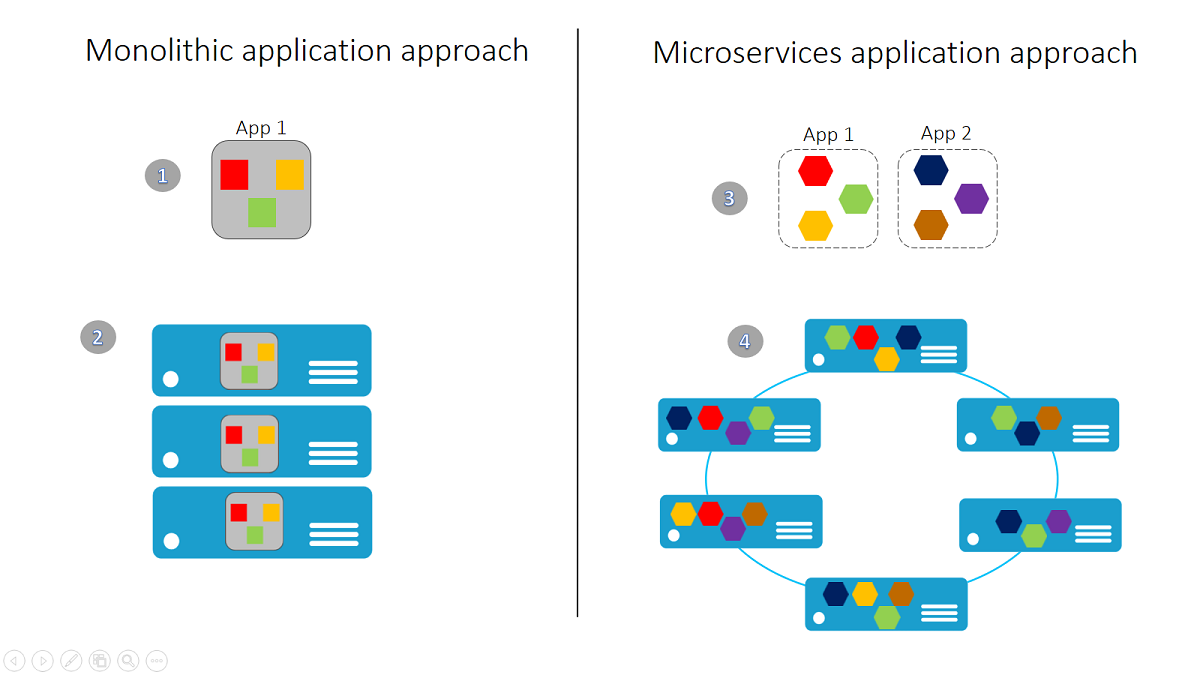
\includegraphics[width=0.9\textwidth]{monolithic_vs_micro}
	\caption[Monolith und Microservice-Architektur] {Monolith und Microservice-Architektur.\cite{msfussell2017azure}}
	\label{fig:mono}
\end{figure}

Abbildung \ref{fig:mono} zeigt eine vereinfachte Gegenüberstellung der beiden Architekturen. Die App 1 ist in drei klassische Funktionen (Web, Business und Data) unterteilt. Die Skalierung (2) kann durchgeführt werden, in dem App 1 über mehrere Server oder VMs geklont wird. 

Bei der Microservice Architektur werden die Funktionen auf unterschiedliche Dienste aufgeteilt. Konkreter könnte dies bedeuten, dass App 1 bei (3) zuständig für eine Benutzerkontoverwaltung ist und App 2 für ein Abrechnungssystem. Die Microservices (4) werden nicht geklont, sondern können unabhängig voneinander bereitgestellt werden. 

\subsection{Monolith vs. Microservices}\label{sec:monolith_vs_microservices}
Aus den vorherigen Abschnitten sind diverse Unterschiede zwischen den Architekturen erkennbar. Nun gilt es festzustellen, für welche Problemstellungen, welche Architektur sinnvoller ist. \cite{wolff2016mic_architectures} \cite{birk2016mic_soa}  

% Tabelle ist nicht ganz Inhaltich richtig

\begin{table}
	\begin{center}
		\begin{tabular}{p{4cm}p{5cm}p{5cm}}
			& Monolithische Architektur & Microservice-Architektur \\ \hline
			Abhängigkeiten & alles in einer Anwendung & entkoppelt, da Prinzip von Modularisierung verwendet wird \\
			Größe & linear steigend & einzelne Services sind klein \\
			Geschwindigkeit Zugriffe & schnell, da alles in einer Anwendung & Zugriffe können länger dauern \\ 
			Deployment & schwieriger desto größer das Projekt, aufgrund von
			\begin{itemize}
				\item Abhängigkeiten  
				\item Größe \end{itemize}
			 & einfach, da Microservices \begin{itemize}
				\item klein und 
			    \item modular sind \end{itemize} \\
			Organisation & leichter, da alles an einem Ort & schwerer, da mehr Domänenlogik (wer macht was?) beachtet werden muss \\
			Legacy-Systeme ablösen & ggf. schwierig, da System sehr verzahnt miteinander & leicht, da Microservices durch neue abgelöst werden können \\
			Technologie & beschränkt & vielfältig \\
			Nachhaltige Entwicklung & wartbar mit Einschränkungen & leicht wartbar \\
			Robustheit & weniger, da ganzes System bei schweren Fehlern abstürzt & sehr, da im Zweifel immer nur ein Service abstürzt \\
			Skalierung & horizontale und vertikale Skalierung, Umsetzung kann sehr komplex werden &  horizontale und vertikale Skalierung \\
			Betrieb & nur ein System & komplex, da mehr Services verwaltet werden müssen
		\end{tabular}
	\end{center}
	\caption[Monolitih vs. Mircoservice-Architektur]{Monolitih vs. Mircoservice-Architektur}
\end{table}



Aus der Tabelle ergeben sich verschiedene Punkte: Der Monolith eignet sich besonders dann sehr gut, wenn die Projekt- sowie Teamgrößen absehbar sind und auch die Technologie entschieden ist. Zusätzlich kann es beim Projektanfang ein Vorteil sein, da die Abhängigkeiten innerhalb des Projektes liegen und so Entwicklungsgeschwindigkeit nicht durch komplizierte Infrastrukturen blockiert wird. 
Ist die Projektgröße allerdings nicht absehbar, treten früher oder später mehrere Schwierigkeiten auf: Zum einen bindet der am Anfang des Projektes festgelegte Technologiestack und die Nutzung oder der Austausch neuer Technologien sind in der Regel mit sehr viel Arbeit verbunden. Des Weiteren führen die anfangs eingegangen Abhängigkeiten zu problemenen im Deployment (A kann erst updaten, wenn B soweit ist) und einem erhöhten Aufwand in der Kommunikation zwischen den Teams (A kann erst beginnen, wenn B xy erledigt hat). \\

Zusätzlich ist die Skalierung von Microservices unabhängiger. Es können sich feingranular Services gesucht werden, welche skaliert werden sollen. Diese benötigen nicht zwingend mehr Hardware (vertikale Skalierung), sondern könnten z.B. auch auf verschiedene Server verteilt werden (horizontale Skalierung). Dies ist bei einem Monolithen natürlich auch möglich, dennoch muss immer der ganze Monolith skaliert werden, welcher zum einen immer mehr Hardware als einzelne Microservices benötigt und zum anderen auch durch die Komplexität in der Regel auch schwerer zu skalieren ist.\cite{wolff2018mic_praxis}   
Als abschließender Punkt ist die Robustheit zu erwähnen: Wenn ein Microservice einen Fehler enthält, stürzt dieser im schlechtesten Fall ab. Im besten Fall übernimmt dieser Service eine weniger wichtige Funktion und der Nutzer bemerkt den Ausfall noch nicht einmal. Beim Monolithen dagegen stürzt die gesamte Anwendungen ab. In der Regel startet so eine Anwendung automatisch neu, jedoch ist betrifft die Downtime alle Nutzer. \\

Aus den genannten Punkten lässt sich schließen, dass eine generelle Aussage, ob eine monolithische oder Microservice-Architektur besser oder schlechter ist, sich nicht treffen lässt. Es kommt immer drauf an, welche Zielsetzung und wie viele Ressourcen für das Projekt festgelegt sind. REWE Digital beispielsweise hat ihr Produkt zuerst als Monolithen gestartet und ist erst später auf eine Microservice-Architektur umgeschwenkt.\cite{rewe2019mic_ppp} Zwei mögliche Gründe könnten dafür sein, dass zum einen ein lauffähiges Produkt schneller mit einer monolithischer Struktur zu erreichen ist, zum anderen ist nicht gegeben, ob ein entwickeltes Projekt überhaupt die Nachfrage erzeugt, so dass eine Microservice-Architektur notwendig ist. Dementsprechend muss abgewogen werden, welche Architektur für welchen Anwendungsfall besser geeignet ist.\cite{wolff2018mic_praxis} 

\subsection{Architektur von Micrsoservices}

% TODO  Taktisches Design wird nicht erwähnt, whrs. auch viele andere Sachen nicht, das muss ich in der Einleitung für DDD noch erwähnen. 

Wie bereits erwähnt, ist die Entkopplung von Microservices ein großer Vorteil gegenüber dem Monolithen. Dennoch ist es sinnvoll Richtlinien, Regeln und/oder Festlegungen zu schaffen, damit die Microservices nicht blockierend oder technologisch unnötig gegensätzlich arbeiten. Die Entscheidungsebene kann global (Makroarchitektur) oder nur für einen einzelnen Services (Mikroarchitektur) gelten.\cite{wolff2016mic_architectures} Welche Festlegungen und mit welcher Strenge diese eingehalten werden müssen, hängt von verschiedenen Faktoren ab, welche technologisch, organisatorisch oder wirtschaftlich motiviert sein können.\cite{rewe2019mic_ppp} \\ 

In dem folgenden Abschnitt wird das Grundprinzip der Software-Modellierungs-Methodik Domain Driven Design untersucht. Zusätzlich wird erläutert, welche Fälle makro- oder microarchitektonisch einzuordnen sind. \\

\subsubsection{Domain Driven Design}

Domain Driven Design (DDD) ist ein Vorgehen mit dem ein Softwaresystem modelliert werden kann. Im Sinne einer Microservice-Architektur kann dies als Werkzeug genutzt werden, um Microservices fachlich einzuteilen.\cite{heise2016ddd} Beim sogenannten \textit{Strategic Design} wird dafür das Softwaressytem in verschiedene \textit{Bounded Contexts} eingeteilt, welche an ein \textit{Domänenmodell} gebunden sind. Ein Domänenmodell bildet die Geschäftslogik ab, d.h. inwiefern einzelne Objekte innerhalb des Kontexts in Relation zueinander stehen, welche Eigenschaften sie haben und wie sich verhalten. Dabei kann ein Domänenmodell - je nach Entwurfsmuster - von einem oder mehreren Bounded Contexts genutzt werden.\cite{wolff2018mic_praxis}  \\

% TODO   ggf. ein paar mehr Worte über die Grafiken verlieren

\begin{figure}[ht]
	\centering
	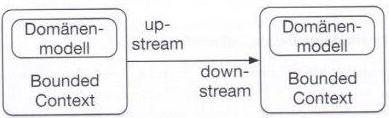
\includegraphics[width=0.5\textwidth]{bounded_context_1}
	\caption[Bounded Contexts mit eigenständigem Domänenmodel] {Bounded Contexts mit eigenständigem Domänenmodell.\cite{wolff2018mic_praxis}}
	\label{fig:bounded_context_with_own_datamodels}
\end{figure}

\begin{figure}[ht]
	\centering
	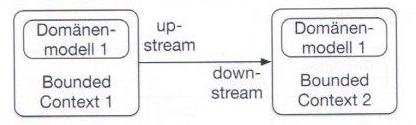
\includegraphics[width=0.5\textwidth]{bounded_context_2}
	\caption[Bounded Context 2 adaptiert das Domänenmodel von Bounded Context 1] {Bounded Context 2 adaptiert das Domänenmodel von Bounded Context 1.\cite{wolff2018mic_praxis}}
	\label{fig:bounded_context_with_copied_datamodel}
\end{figure}

\begin{figure}[ht]
	\centering
	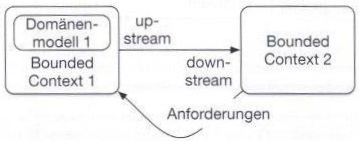
\includegraphics[width=0.5\textwidth]{bounded_context_3}
	\caption[Bounded Context 2 erhält ein auf ihn zugeschnittenes Domänenmodel von Bounded Context 1] {Bounded Context 2 erhält ein auf ihn zugeschnittenes Domänenmodel von Bounded Context 1.\cite{wolff2018mic_praxis}}
	\label{fig:bounded_context_with_custom_datamodels}
\end{figure}

Wolff verdeutlicht das Prinzip von Bounded Contexts mit Hilfe von vier Microservices, welche einen Onlineshop repräsentieren: \textit{Suche}, \textit{Check Out}, \textit{Inkasso} und \textit{Lieferung}. Während das Datenmodell der Suche detaillierte Informationen über die Produkte enthält, reicht es im Warenkorb (hier Check Out), wenn ggf. nur der Produktname gespeichert wird. Bei Inkasso ist es ähnlich: An dieser Stelle sind Zahlungsdaten des Benutzers relevant, während bei Lieferung die ggf, nur Adresse notwendig ist.\cite{wolff2018mic_praxis} An diesem Beispiel wird deutlich, dass zwar von selben Begrifflichkeiten wie Benutzer, Produkt usw. gesprochen wird, allerdings jeder Service sein eigenes Domänenmodell hat. Durch diese Technik, was dabei hilft, eine saubere Microservice-Architecktur zu erstellen.\cite{wolff2018mic_praxis} \cite{heise2016ddd} \\

Neben der fachlichen Trennung bildet DDD auch die Kommunikation zwischen Kontexten ab. Dabei wird grundsätzlich vom \textit{up-stream} (vorgeschaltet) und dem \textit{down-stream} (nachgeschaltet) gesprochen.\cite{wolff2018mic_praxis}. Der up-stream stellt dem down-stream Informationen bereit. Wie dies technisch umgesetzt ist, also ob der down-stream nachfragt oder der up-stream aktiv Daten schickt, ist frei wählbar. \\

Nach dem Anwenden von DDD sollte die Struktur der Software erkennbar sein: D.h. welche Art Microservices werden benötigt und iwiefern sie mit anderen in Abhängigkeiten bzw. Kommunikation stehen.   

\subsubsection{Macro- und Mikroarchitektur}

Wenn durch das DDD entworfen wird, welche Microservices voraussichtlich benötigt werden, ist es sinnvoll einen Art Bauplan zu verfassen, welcher impliziert, an welche Regeln sich ein Microservice halten muss. Diese Regeln können wie bereits erwähnt auf globaler Ebene getroffen werden, d.h. sie gelten für alle Services (Makroarchitektur) oder sie gelten nur im Microservice selber (Microarchitektur). REWE Digital unterscheidet dabei zwischen \textit{Must}, \textit{Should}, \textit{Could}. D.h. es gibt Regeln, die Microservices erfüllen müssen wie z.B. das Kommunzieren über REST oder das Implementieren eine einheitlicher Autorisierung.\cite{rewe2019mic_ppp} Andere Regeln dagegen sind viel mehr Richtlinien (should) oder komplett optional (could). Das Ziel ist stets, dass durch die makroarchitektonischen Entscheidungen nicht die Vorteile von Microservices beschnitten werden.\cite{wolff2018mic_praxis}\cite{irakli2016mic_arc}. \\

Es gibt verschiedene Einflussfaktoren wie sich die Makroarchitektur für ein Unternehmen definiert: Zum einen empfiehlt es sich ein Gremium zu gründen, welches sich stetig mit den Regeln der Makroarchitektur auseinandersetzt, sie entsprechend erweitert, überarbeitet und die getroffenen Entscheidungen auch immer begründen kann.\cite{wolff2018mic_praxis} Zum anderen besteht immer ein technischer Einfluss\cite{wolff2018mic_praxis}:
\begin{itemize}
	\item Gewählte Technologien müssen in die Infrastruktur des Unternehmens passen: Angenommen die Auslastung eines Microservices muss überwacht werden und dies wird firmenweit mit Tool A erledigt, dann wäre es sehr aufwendig, wenn der besagte Service nur eine Schnittstelle für Tool B anbietet und der nächste Service nur für Tool C. Dies würde einerseits sehr unübersichtlich werden und andererseits viel Aufwand bedeuten. 
	\item Technologien sind immer von dem Personal abhängig: Gerade wenn Unternehmen klein bis mittelständig sind, emphielt es sich Technologien zu nutzen, die mehrere Entwickler beherrschen, um Inselwissen zu reduizieren. 
	\item Ebenfalls können gezielt strategische Entscheidungen getroffen werden, z.B. wenn ein Unternehmen die Dateninfrastruktur zu einem Cloudanbieter auslagern möchte, hat dies entsprechende makroarchitekonisches Auswirkungen.
\end{itemize}

Basierend auf Wolff und Nadareishvili ist folgende Tabelle entstanden, welche einen Überblick darüber gibt, wie gängige Entscheidungspunkte einzuordnen sind. \cite{wolff2018mic_praxis}\cite{irakli2016mic_arc}\cite{rewe2019mic_ppp}

\begin{table}
	\begin{center}
		\begin{tabular}{p{5cm}p{5cm}p{5cm}}
			& Mikroarchitektur & Makroarchitektur \\ \hline
			Programmiersprache &  x & x  \\
			Datenbank & x & x \\
			Look and Feel (UI) & x  & x  \\
			Dokumentation & x & x  \\
			Datenformat &   & x \\
			Kommunikationsprotokoll &   & x \\
			Authentifizierung &  & x \\
			Integrationtests &  &  x \\
			Autorisierung & x  &  \\
			Unittests & x  &  \\
			Continuous-Delivery-Pipeline & x &  \\
		\end{tabular}
	\end{center}
	\caption[Entscheidungen Micro- und Macroarchitektur]{Entscheidungen Micro- und Macroarchitektur}
\end{table}

In der Tabelle sieht man, dass gerade die ersten Punkten sehr von der Unternehmenskultur und den technischen sowie personellen Freiheiten abhängt. In der Theorie sollte die Programmiersprache sinnvoll für jeden Microservices gewählt werden, dennoch ergibt es auch Sinn einen Pool an Programmiersprachen auf Makroebene zu definieren, um Inselwissen zu reduzieren und nachhaltige Codequalität zu gewährleisten. Ähnliches gilt beispielsweise für die Wahl der Datenbank: Ist bereits eine globale Infrastruktur für Datenbank X geschaffen, sollte diese nicht ohne weiteres aufgebrochen werden, nur weil es technisch möglich ist. \\

Bei der Dokumentation sowie beim Look \& Feel ist es sinnvoll, globale Richtlinien zu definieren, damit klar ist, wo bei jedem Microservices die Dokumentation zu finden ist oder wie ein User Interface grundsätzlich angeordnet und gestaltet werden soll. Dennoch können diese Punkte im Detail je nach Microservice abweichen. \\

Ein Kommunikationsprotokoll (z.B. REST) sowie Datenformate (z.B. JSON) sollten festgeschrieben werden.\cite{rewe2019mic_ppp} \cite{wolff2018mic_praxis} Als Grund wird zum einen das Vermeiden von technischen Mehraufwand angegeben, zum anderen sind Microservices zwar eigenständig deploybare Einheiten, dennoch sollten sie technisch zum Gesamtsystem passen und nicht dagegen arbeiten. \\

Während die Authentifzierung (um wen handelt es sich) einmalig festgelegt werden sollte, liegt die Überprüfung der Autorisierung (was darf der Benutzer) in jedem Microservice selbst. Die Alternative wäre, dass jede eingehende Anfrage noch einmal geprüft wird, was zu unnötig hohem Traffic und Verzögerungen führen würde.  \\

Die hier erarbeitete Tabelle ist an dieser Stelle nicht als feststehendes Manfifest für alle Unternehmen zu verstehen, sondern als neutral betrachtete, sinnvolle Einordnung. Natürlich können architektonische Entscheidungen stark vom jeweiligen Anwendungszweck abhängen. \\

Die Tabelle zeigt lediglich allgemeine Beispiele und ist nicht als vollständig zu betrachten. Nicht aufgeführt ist beispielsweise der Umgang mit Konfigurationsdateien, Monitoring oder Logging. Dies liegt unter anderem daran, weil es auf Projekte oder von dem Microservice abhängt: Beim Monitoring könnte zum Beispiel global entschieden werden, \textit{wo} Metriken abgelegt werden bzw. mit \textit{welcher} Technologie gearbeitet wird. Aus microarchitektonischer Sicht könnten die Services selbst entscheiden, \textit{was} gemessen wird.  \\

Ebenso beim Deployment: Es gibt zahlreiche Methoden, um neue Updates bereitzustellen wie z.B. mittels Docker, Kubernetes oder indivudelle Installationsskripte.\cite{wolff2018mic_praxis} Welche Technologie sich durchsetzt, muss anhand der Anforderung entschieden werden. \\

Aus den erarbeitenten Punkten lassen sich Vor- und Nachteile ableiten, zwischen denen abgewogen werden muss. Vorteile für microarchitektonische Entscheidungen sind ein sehr hohes Maß an Flexibilität und eine hohe Unabhängigkeit im Gesamtsystem, was grundsätzlich das Ziel von Microservices ist. Dies wiederum kann dazu führen, dass Entwicklungsoverhead oder Inselwissen entsteht. Ebenfalls könnten Punkte wie z.B. das \textit{Look \& Feel} oder die \textit{Dokumentation} darunter leiden.  \\

Macroarchitektonische Entscheidungen haben zum Vorteil, dass es Regeln gibt, welche die Entwicklung vereinfachen sollen und gegebenfalls die Nachteile der Microarchitektur kompensieren können. Auf der anderen Seite schränken macroarchitekonische Entscheidungen ein. Zusätzlich müssen sie organisch, z.B durch ein extra dafür geschaffenes Gremium, durchgesetzt und werden.\cite{wolff2018mic_praxis} Im Gesamten lässt sich daraus schließen, dass sehr genau abgewogen werden muss, welche Entscheidungen global oder individuell entschieden werden. Grundsätzlich gilt, dass jede Entscheidung begründbar sein muss.    

\subsection{Kommunikation}

Bei einem Monolithen wird eine Abfrage über eine Route gestellt, woraufhin die Anwendung entsprechend mit der Bearbeitung beginnt. Da die gesamte Datenhaltung an einer Stelle ist, sind alle Daten bekannt und abrufbar. Wichtiger noch: Die Daten sind konsitent. \\

Microservices sind diesbezüglich herausfordernder. Es müssen verschiedene architektonische Entscheidungen getroffen werden, wie z.B. ob es einen zentralen Service gibt, welcher alle Anfragen weiterleitet (\textbf{API Gateway}) oder ob jeder Service einzeln erreichbar ist. Ebenfalls sollte auch begründbar entschieden werden, ob eine synchrone,  asynchrone oder möglicherweise eine hybride Kommunikation verwendet wird. 

In den folgende Unterkapiteln werden Vor- und Nachteile der verschiedenen Kommunikationsarten für Microservices mit einem Schwerpunkt auf Unabhängigkeit (Entkopplung) und Datenkonsitenz untersucht.

% Problem beschreiben, warum kann man nicht einfach alles über REST klären
% Beispiel aus Microservice in Action: Zwei Aufrufe gehen gut, der dritte nicht, ungewollten State.
% ggf. das 2PC Protokoll bemerken, dass das eine Lösung ist, aber auch nicht funktioniert: Gegengründe aufführen
%was ist die Lösung: Event Based

\subsubsection{Synchrone Kommunikation}\label{sec:synchrone_kommunikation}

Wenn ein Microservice bei der Bearbeitung einer Anfrage selbst eine weitere Anfrage an einen anderen Microservice stellen muss und auf das Ergebnis wartet, spricht man von synchroner Kommunikation.\cite{wolff2018mic_praxis} 

Anhand dieser Definition lässt sich folgendes Szenario darstellen (siehe Abbildung \ref{fig:synchrone_kommunikation_microservices}). 

\begin{figure}[ht]
	\centering
	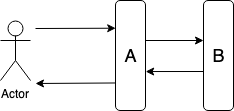
\includegraphics[width=0.5\textwidth]{synchrone_kommunikation_microservices}
	\caption[Synchrone Kommunikation] { Synchrone Kommunikation}
	\label{fig:synchrone_kommunikation_microservices}
\end{figure}

Der Actor fragt bei Microservice A an, welcher diese Anfrage bearbeitet und schließlich an B weiterleitet. B verarbeitet die Anfrage und antwortet, schließlich kann auch A antworten. Aus diesem Ablauf lässt sich festhalten, dass die übertragenden Daten aktuell sind. D.h. der Actor erhält definitiv konsistente Daten, was positiv zu vermerken ist. Problematischer dagegen ist die Abhängigkeit, welche entsteht. Sollte B nicht erreichbar sein, läuft A in einen Timeout und ist blockiert. Einerseits ließe sich argumentieren, dass genau dies passieren soll, schließlich scheint es einen Fehler zu geben. Aber angenommen A wäre ein Service zum Erstellen von Rechnungen und B ein Service zum Sammeln von Daten. A möchte B infomieren, dass eine Rechnung erstellt wurde, ist aber blockiert. Die Operation eine Rechnung zu erstellen hätte höhere Priorität als es statisch zu erfassen. Nach den aufgestellen Definitionen aus \ref{sec:monolith_vs_microservices} für Microservices wird die Entkopplung, Modularität und Robustheit des Systems verletzt, da A nicht weiterarbeiten kann.\cite{wolff2018mic_praxis} \cite{bruce2019mic_in_action}  

Bläht man das Beispiel auf, so dass weitere Services statistische Daten erfassen wollen, würden zahlreiche Microservices ausfallen (siehe Abbildung \ref{fig:snyn_com_dependencies}). \\

\begin{figure}[ht]
	\centering
	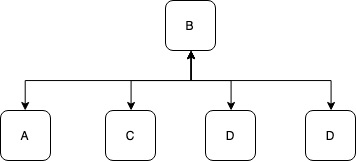
\includegraphics[width=0.5\textwidth]{snyn_com_dependencies}
	\caption[Abhängigkeiten in synchroner Kommunikation] { Abhängigkeiten in synchroner Kommunikation}
	\label{fig:snyn_com_dependencies}
\end{figure}

Die Microservices können auch nicht auf eine Notfallstrategie (\textbf{Fallback}) zurückgreifen. Angenommen wenn Serivce B nach x Sekunden nicht erreichbar ist, wird die ursprüngliche Abfrage durch A weiter abgearbeitet, um nicht zu blockieren. Nun müsste eine andere Logik dafür sorgen, dass die Daten, die nicht übertragen werden konnten, zu einem anderen Zeitpunkt übertragen werden. In diesem Moment herrscht keine Konsistenz mehr vor, was aber ein großer Vorteil an synchroner Kommunikation ist. \\

Betrachtet man das Beispiel andersherum und nimmt an, dass jeder Service seine Datenhaltung soweit aufspreizt, dass jeder Service die Statistiken führt, ist es nur eine Frage der Zeit, bis weitere Felder gespeichert werden müssen. Überspitzt formuliert, würde jeder Service alles speichern, was gegen die Absicht von Bounded Contexts arbeiten würde.\cite{wolff2018mic_praxis} \\

Auch nicht zu vernachlässigen, ist die Geschwindigkeit mit der die Abfragen abgearbeitet werden können. Möglicherweise muss B in einem anderen Szenario noch mit C kommunizieren. Die Anfrage würde sich über drei Services erstrecken, was zusätzliche Latenzzeiten mit sich bringt.\cite{wolff2018mic_praxis} \\   

Ebenfalls entsteht durch jede Schnittstelle eine fachliche Abhängigkeit geschaffen.\cite{bruce2019mic_in_action} Die Anfragen von den Microservices A, C, D, E müssen der Schnittstellendefinition von B entsprechen. Änderungen führen gegebenenfalls zu Fehlern und weiteren Abhängigkeiten. Wie diese Problematik gelöst werden könnte, wird \ref{sec:asynchrone_kommunikation} beschrieben.

\subsubsection{Asynchrone Kommunikation}\label{sec:asynchrone_kommunikation}

Wie bereits beschrieben, wird bei der synchronen Kommunikation auf weiterführende Abfragen gewartet. Die asynchrone Kommunikation wartet nicht auf Antworten von weiteren Services, sondern trifft Annahmen über etwaige Systemzustände.\cite{wolff2018mic_praxis} Um Annahmen zu treffen, existieren je nach Anwendungsfall verschiedene Strategien:

\begin{enumerate}
\item{ Ein Microservice kann replizierte Daten vorhalten. Angenommen ein Artikel soll rausgeschickt werden: Der dafür verantwortliche Service benötigt die Anschrift des Kundens, aber nicht weitere Daten wie Geburtsdatum, Zahlungsmethode oder ähnliches. Dementsprechend werden nur relevante Daten repliziert vorgehalten. Eine Herausforderung ist es, dass diese replizierten Daten stets mit den Originaldaten übereinstimmen. Schließlich kann sich eine Anschrift ändern.\cite{wolff2018mic_praxis}}

\item{Ggf. muss nur ein weiterer Service informiert werden wie der Service B aus Abschnitt \ref{sec:synchrone_kommunikation}, welcher Statistiken erfasst. In dem Szenario der asynchronen Kommunikation würde die Abfrage gestellt werden ohne das Ergebnis abzuwarten, da es schlichtweg nicht relevant ist. Die Herausforderung hier ist, zu gewährleisten, dass die Abfrage auch in Fehlerfehlen früher oder später zugestellt wird.}
\end{enumerate}

Aus den Strategien ergeben sich Anforderungen an die Kommunikationsstruktur: Es muss gewährleisten sein, dass fehlerhafte Abfragen erneut übermittelt werden und ebenfalls wird eine Struktur benötigt, die dafür sorgt, dass replizierte Datensätze stets mit aktuellen Daten befüllt sind. Dies lässt sich durch sogenannte Events erreichen.\cite{bruce2019mic_in_action}.\cite{wolff2018mic_praxis}  \\

Die folgende Abbildung \ref{fig:microservices_bus} verdeutlich das Prinzip von Events und deren Infrastruktur: 

\begin{figure}[ht]
	\centering
	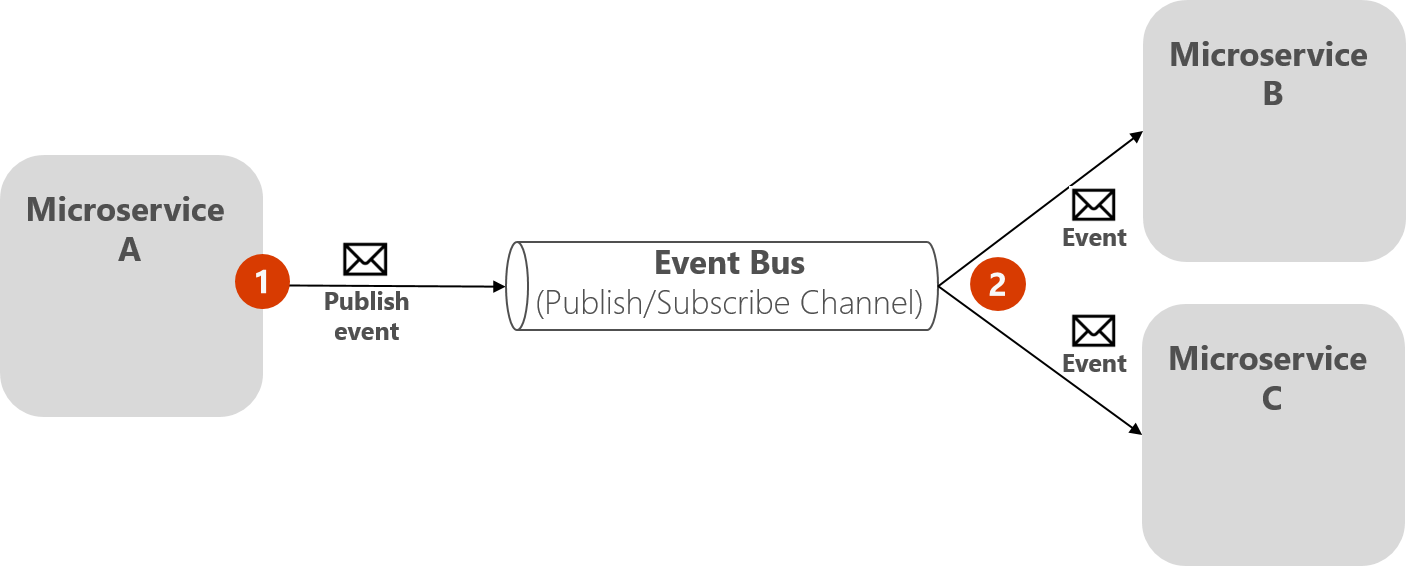
\includegraphics[width=0.5\textwidth]{microservices_bus}
	\caption[Eventbus mit Events] { Eventbus mit Events\cite{cesardelatorre2018azure}}
	\label{fig:microservices_bus}
\end{figure}

In dieser Abbildung haben Microservice B und C das Event x beim Ergeinisbus (\textbf{Event Bus}) abonniert (\textbf{subscribed}). D.h. Microservice A veröffentlicht (\textbf{published}) eine Änderung, woraufhin B und C informiert werden. B und C können nun ihren Datenbestand aktualisieren und halten so die aktuellen Daten vor. Parallel kann der Microservice A seine Abfrage ganz normal weiterführen. Der Eventbus ist dementsprechend ein Vermittler (\textbf{Message Broker}), welcher garantiert, dass die Nachrichten übertragen werden. Dieser sollte mit etwaigen Fehlerfällen (z.B. C ist nicht erreichbar) umgehen können und eine spätere Übertragung garantieren. \cite{cesardelatorre2018azure}\cite{wolff2018mic_praxis} \\

Aus diesem Modell ergibt sich ein weiterer Vorteil, nämlich dass die Microservices entkoppelt sind. Es wird keine REST-Schnittstelle definiert, welche eine gewissen Fachlogik vorgibt. Ebenfalls können mehrere Services auf ein Event hören. Wolff warnt allerdings davor Events unnötig aufgebläht zu gestalten: Zum einen werden schnell Daten übermittelt, die nicht für alle Abonnenten (\textbf{Subscriber}) relevant sind und zum anderen entspräche dies nicht dem Prinzip vom DDD. \\

% Verhindern, dass Message Broker nicht erreichbar ist, durch
% - Der Message Broker sollte redundant laufen, wodurch schonmal eine hohe Wahrscheinlichkeit existiert, dass er erreichbar ist
% - Häufig ist es bei den Systemen so, dass man bspw. Innerhalb einer DB Transaktion in eine Tabelle schreibt, welche Events an den Broker dispatcht werden sollen. Und dann gibt es einen Background Task, der regelmäßig schaut, welche Events noch nicht an den Broker geliefert wurden und sendet die dahin
%- Wenn das fehlschlägt, dann versucht er es später wieder
%- Und das mit der Transaktion hat den Vorteil, dass eventuelle Änderungen in der DB garantiert  klappt oder beides (auch Speichern d. Events in einer Dispatcher Tabelle) fehlschlägt. Aber keine Inkonsistenzen

Zusätzlich sollte beachtet werden, dass Microservices so gestaltet werden, dass sie idempotent sind. In diesem Zusammenhang bedeutet dies, dass falls ein selbes Event zweimal übertragen wird, der Microservice die Aktion nicht zweimal ausführt. D.h. eine Mehrfachausführung führt zu dem selben Ergebnis wie eine einzige Ausführung. Wenn z.B. eine Rechnung versendet werden soll, ist garantiert, dass diese nur ein einziges Mal versendet wird.\cite{wolff2018mic_praxis} \\

\subsubsection{Abwägung asynchrone vs. synchrone Kommunikation}

Aus den zwei vorherigen Abschnitten ergibt sich folgende Aufstellung (siehe Tabelle \ref{tab:sync_vs_async_table}).

\begin{table}[H]
	\begin{center}
		\begin{tabular}{p{1,5cm}p{5cm}p{5cm}}
			& synchrone Kommunikation & asynchrone Kommunikation \\ \hline
			 Vorteile
			&
				\begin{itemize}
					\item Jederzeit Konsitent
					\item Paradigma ist Entwicklern bekannt\cite{wolff2018mic_praxis}
				\end{itemize} 
			& 
				\begin{itemize}
					\item Entkoppelt durch Events 
					\item Flexibilität, da ein Event mehre Services erreichen kann
					\item Nachrichtenempfang garantiert (ggf. mit Verzögerung)
					\item Absicherung gegen Ausfall
				\end{itemize} 
  			\\
			Nachteile
		  &
 			  	\begin{itemize}
				 	\item Anfälligkeit durch Abhängigkeiten 
				 	\item Erweiterbarkeit ist schwerer, da fachliche Abhängigkeiten
				 	\item Ggf. lange Netzwerkzeiten
				 \end{itemize}
		  & 
		 	\begin{itemize}
		 		\item nicht jederzeit garantiert konsistent
		 		\item Idempotenz muss beachtet werden
	 		\end{itemize}  \\
		\end{tabular}
	\end{center}
	\caption[synchrone vs. asynchrone Kommunikation]{synchrone vs. asynchrone Kommunikation}
	\label{tab:sync_vs_async_table} 
\end{table}

Es lässt sich feststellen, dass die Vorteile einer asynchrone Kommunikation für Microservices überwiegen und auch diese wird empfohlen.\cite{wolff2018mic_praxis}\cite{bruce2019mic_in_action} Allerdings ist die Kommunikation nicht dogamtisch zu betrachten, sondern sollte je nach Projekt und Anwendungsfall entschieden werden. Synchrone Kommunikation bietet sich nämlich gerade dann an, wenn der Datenbestand definitiv konsistent sein sollen. \\

Das sogenannte CAP-Theoreom beschreibt die Abwägung, welche man in verteilten Systemen bei der Auswahl der Kommunikation treffen muss. CAP bedeutet:
	\begin{itemize}
		\item Consistency (Konsistenz): Die Daten in einem verteilten System sind konsistent.
		\item Availability (Verfügbarkeit): Die Verfügbarkeit für alle Systeme ist gegeben. 
		\item Partition Tolerance (Partitionstoleranz): Das Gesamtsystem arbeitet auch weiter, wenn Teile davon ausfallen. 
	\end{itemize}  

In einem verteilten System können immer nur zwei von den drei Bedinungen erfüllt sein.\cite{wolff2018mic_praxis}. Sofern Konsistenz gewährleistet soll, müssen alle dienste stets verfügbar sein. Damit kann der Punkt Partitionstoleranz nicht erfüllt sein. Umgekehrt: Wenn die Partitionstoleranz garantiert ist, z.B. dadurch dass Services ihre eigene Datenhaltung besitzen, ist zwar prinzipiell auch die Verfügbarkeit gegeben, aber nicht die Konsistenz. \\

Dementsprechend ist es sinnvoll sich die Anforderungen, welches man an sein System hat zu überlegen und sich aufgrund dieser Grundlage zu entscheiden, welche Kommunikationsart implementiert werden soll. 

\subsubsection{API-Gateway}

Umso mehr Services aufgesetzt werden, desto komplexer ist es, die Übersicht über alle zu behalten. Eine Abhilfe im Routing bietet ein sogeanntes API-Gateway. Ein API-Gateway ist der einzige Einstiegspunkt für den Nutzer (\textbf{Client}). Von dort wird er weitergeleitet, ohne die Routen von einzelnen Services zu kennen. 

\begin{figure}[ht]
	\centering
	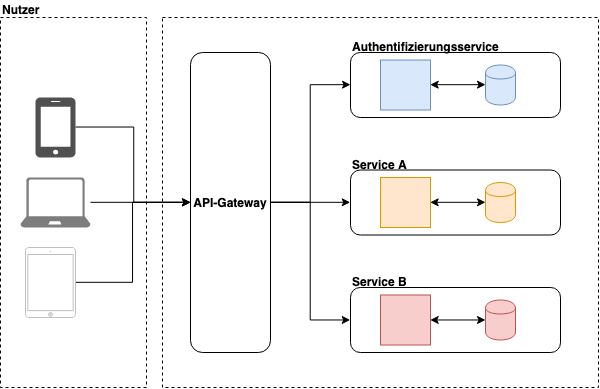
\includegraphics[width=0.6\textwidth]{api_gateway}
	\caption[Prinzip API-Gateway] { Prinzip API-Gateway }
	\label{fig:api_gateway}
\end{figure}

Abbildung \ref{fig:api_gateway} zeigt deutlich wie die Clients über das Gateway kommunizieren, welches anschließend an die entsprechenden Services weiterleitet. Wenn APIs eine hohe Auslastung haben, würde man mehrere Instanzen von einem API-Gateway erstellen. Ein sogenannter Load Balancer wäre der Einstiegspunkt für die Clients. Dieser würde die Anfragen sinnvoll an die API-Gateway-Instanzen verteilen, so dass keine Überlastung entsteht.\cite{oracle} \\

API-Gateways haben neben dem einzelnen Einstiegspunkt noch weitere Vorteile: 
\begin{itemize}
	\item Höhere Sicherheit, das einzelne Services nicht sichtbar und nur über das Gateway zu erreichen\cite{bruce2019mic_in_action}
	\item Authentifizierung kann bereits im Gateway ausgeführt werden, dies führt zu weniger Last für einzelne Microservices.\cite{wolff2018mic_praxis}
	\item Zentralisiertes Logging, Caching, Monitoring, Mocking sowie eine zentralisierte Dokumentation ist möglich.\cite{wolff2018mic_praxis}
\end{itemize}  

Ein Nachtteil in der Struktur des API-Gateways ist, dass die Abfragen länger sind, da sie immer erst über das Gateway gehen.\\

\subsection{Authentifizierung und Autorisierung}

Beim Monolithen ist architektonisch klar, dass die Authentifizierung und Autorisierung innerhalb des Monolithen stattfindet. Im Bereich der Microservice Architektur existieren verschiedene Szenarien, wie man eine Authentifizierung sowie Autorisierung gestalten kann.\cite{bruce2019mic_in_action} \\

\textbf{Authentifizierung}: Identifiziert, wer jemand ist. Z.B. Nutzer A, der sich durch Benutzername und Passwort registriert hat.\cite{bruce2019mic_in_action}
\textbf{Autorisierung}: Bestimmt, wie viel ein Nutzer darf. Nutzer A hat eine Rolle, welche ihn berechtigt gewisse Aktionen durchzuführen.\cite{bruce2019mic_in_action}

Es emphielt sich die Autorisierung in den Microservices ansich zu überprüfen, da diese den entsprechenden Datenbestand haben. Um unnötige Last zu verhindern, kann die Validität - ob es sich überhaupt um einen gültigen Request handelt - bereits im API-Gateway überprüft werden. Die Authentifizierung dagegen sollte in einem eigenen Service oder ins API-Gateway verlagert werden.\cite{rewe2019mic_ppp}\cite{richardson2019mic_pattern} Zu empfehlen ist, dass die Authentifizierung an einer zentralen Stelle durchgeführt wird, um Redundanz und fehlerhafte Implementierungen zu verhindern. \\

Die Idee ist, dass der Benutzer nach dem Anmelden ein Security-Token erhält, welches verwendet wird, um sensible Anfragen zu verifizieren. Zum einen gibt es die Möglichkeit ein Token auszustellen, welches beim Auslesen verschlüsselt ist (opaque Token) und zum anderen auf ein offenen Standard namens Json Web Token (JWT, transparent Token) zu setzen. Das opaque Token hat den großen Nachteil, dass es zusätzliche Performance sowie Latenz verursacht und nur synchron entschlüsselt werden kann.\cite{richardson2019mic_pattern} \\

Das JWT wird beim Ausstellen signiert, um die Echtheit zu gewährleisten. Während die Nachteile des opaque Token hier nicht auftreten, ist ein anderes Problem, dass ein JWT nach Ausstellung nicht widerrufen werden kann. Theoretisch wäre es dauerhaft gültig, weshalb Ablauflaufzeiten gesetzt werden. Dies wiederum impliziert, dass der Client dafür sorgen muss, immer rechtzeitig ein neues Token anzuforden. Für solche und weitere Logiken exisitiert bereits ein Sicherheitsstandard namens OAuth2, welcher empfohlen wird zu verwenden.\cite{richardson2019mic_pattern} \\

Ziel bei OAuth2 ist unter anderem Autorisierungen zwischen verschiedene Anwendungen zu erlauben. Ursprünglich wurde das Authentifizierungsprotokoll so entworfen, dass Drittanwendungen Zugang zu Informationen erhalten, ohne dass Passwörter weitergeleitet werden müssen.\cite{richardson2019mic_pattern}  Beispielsweise wird OAuth2 verwendet, wenn Benutzer sich über ihren Facebook-Account bei Drittplattformen anmelden. Die Drittplattformen können natürlich nicht das Facebook-Passwort einsehen, erhalten aber je nach Anwendungsfall Zugriff auf verschiedene Ressourcen (z.B. Lesezugriff auf die E-Mail-Adresse und/oder Konakte, Schreibzugriffe zum Teilen von Nachrichten usw.). \\

Da OAuth2 ein sehr komplexes und umfangreiches Thema ist, wird im Folgenden nur ein häufig verwendetes Grundprinzip erklärt. \\

Um die Abbildung \ref{fig:password_grant} besser zu verstehen, sind folgende Definitionen hilfreich:\cite{richardson2019mic_pattern}\\

\textbf{Authorization Server}: Authentifiziert den Benutzer und gibt ein Access sowie Refresh Token raus.\\

\textbf{Access Token}: Durch ein Access Token erhält man Zugriff auf den Resource Server. Das Format ist Abhängig von der jeweiligen Implementierung, eine bereits genannte Möglichkeit wäre JWT. Der Access Token ist zeitlich begrenzt gültig. \\

\textbf{Refresh Token}: Ein Token welches langlebig ist, also eine lange Gültigkeit besitzt. Dieses kann allerdings im Gegensatz zum Access Token widerrufen werden. Ebenfalls wird es verwendet, um ein neues Access Token vom Authorization Server anzufordern. Dafür ist keine Übergabe der Benutzerdaten nötig.\\ 

\textbf{Resource Server}: Eine Resource auf die nur zugegriffen werden kann, wenn ein valides Access Token vorliegt, dies könnte z.B. ein Micoservice sein.\\ 

\textbf{Client}: Ein Client möchte Zugriff auf den Resource Server. Clients können beispielsweise Drittanwendungen, Webanwendungen oder mobile Applikationen sein.  \\ 

\textbf{Client}: Ein Client möchte Zugriff auf den Resource Server. Clients können beispielsweise Drittanwendungen, Webanwendungen oder mobile Applikationen sein. Sie werden auch Resource Owner genannt. 

\begin{figure}[H]
	\centering
	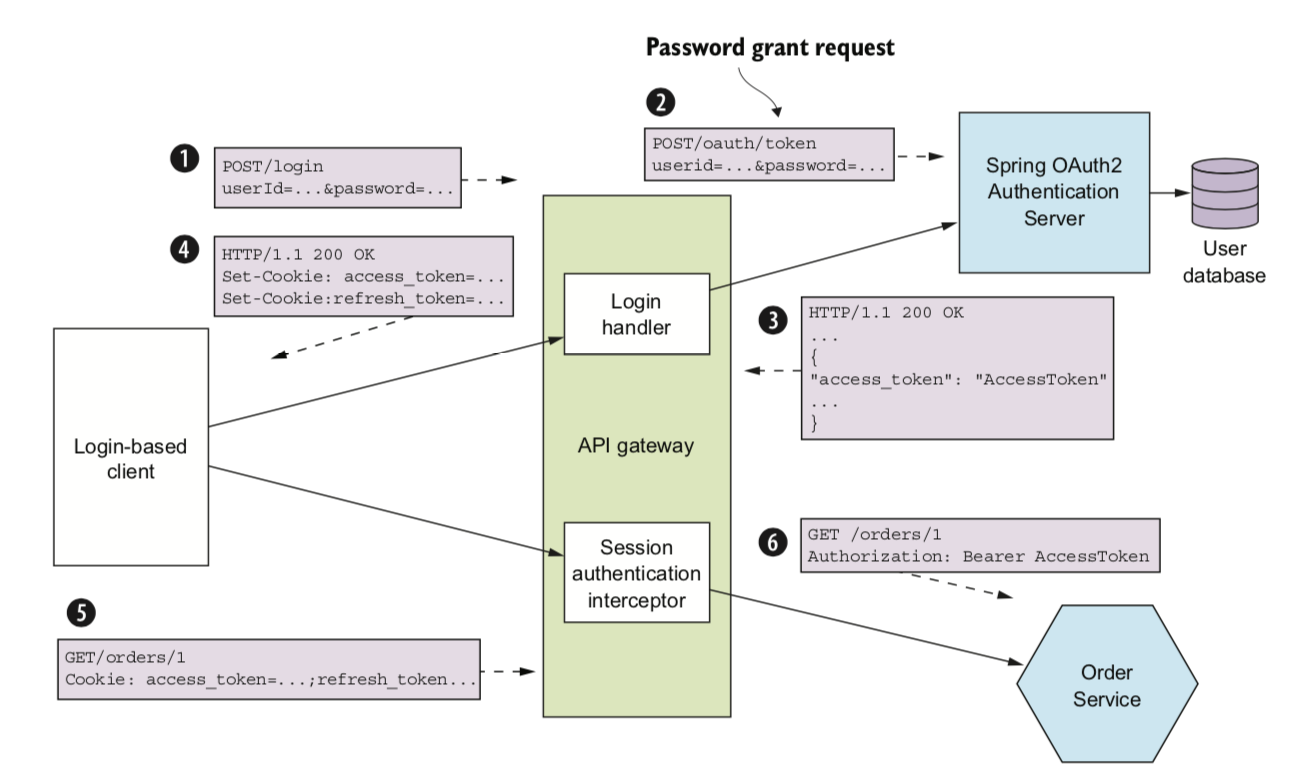
\includegraphics[width=0.7\textwidth]{password_grant}
	\caption[Ablauf eines password grants] { Ablauf eines sogenannten `password grant`\cite{richardson2019mic_pattern} }
	\label{fig:password_grant}
\end{figure}

Die Abbildung \ref{fig:password_grant} zeigt einen Ablauf, bei dem ein Client sein Usernamen und Passwort übermittelt (1). Diese Anfrage wird von dem API-Gateway weitergeleitet an einen Authorization Server (2). Wurde der Nutzer gefunden, wird ein Access und Refresh Token über das API-Gateway (3) an den Nutzer übermittelt (4). Mit der entsprechenden Authorisierung ruft der Client seine Bestellungen (5) ab. Dieser Request wird entsprechend von dem API-Gateway weitergeleitet (6). \\

Neben dem \textit{password grant Flow} existiert auch der sogenannte \textit{client credentials grant Flow}. Dieser funktioniert ähnlich, nur dass nicht Username und Passwort übertragen werden, sondern der Anwendungen durch gemeinsam bekannte Daten zwischen Anwendungen und Authorization Server vertraut wird. Den \textit{client credentials grant Flow} sollte man verwenden, wenn eine Applikation Ressourcen aufrufen möchte, die außerhalb eines User-Kontextes liegen, d.h. es handelt sich in der Regel um recht allgemeine Daten.\cite{oauth2}\cite{richardson2019mic_pattern} \\

Aufgrund dieser Grundlage wird im Konzept VERLINKUNG-EINFÜGEN herausgearbeitet, welche Möglichkeiten zur technischen Umsetzung dieser Flows bereitstehen. 

\subsection{Docker}

Über Docker können Anwendungen innerhalb eines Containers laufen. Ein Container ist vergleichbar mit einer sehr leichtgewichtigen, modularen virtuellen Maschine.\cite{RedHat} Docker in der Tiefe aufzuarbeiten, würde den Umfang dieser Arbeit überschreiten. Dennoch wird im Folgenden erläutert, warum speziell Docker sich sehr gut für Microservices eignet und wie das Wirkungsprinzop von Docker ist. \\


Löst Schwierigkeiten: Portkonfiguration, Ressourcentrennung (wenn alle Projekte sich ein Betriebssystem teilen, wer gewährleistet, dass Prozesse sich nicht behindern)

Vorteile zur VM (Microservice hat eigenes Betriebssystem, was auf der selben Hardware läuft): Performance schlechter, weil VM dem Betriebssystem die Illusion gibt, dirket auf echter Hardware zu laufen.
Jeder Microservice eigene Instanz = Viel RAM + viel Speicherplatz, da gesamtes Betriebssystem

=> Docker ist leichtgewichtige Variante, zwar kein ganz so starke Isoloation, aber ähnlich wie ein Prozess (kein signifikanter Overhead): 

teilen sich Kernel, nutzen eigenes Netzwerkinterface => flexible Portfreigaben
ist durch eine Schichtenarchitektur speicherplatz schonend, da Ressourcen wiederverwendet werden können, gleicht einem Prozess von der Leistung her. Deshalb kann man ohne Probleme 100 Container auf einem Laptop laufen lassen im Gegensatz zu 100 virtuellen Maschinen. 

Ablauf erklären
Dockerfile beschreibt Image
Container (aktive Instanz vom Image)
Image (Speicherabbild von Container) 
Image wird in Repository gespeichert
Docker-Host: 

Bild zeigen, erklären, alternative erwähnen WAR Images, auf mehr wird nicht eingegangen. 